\RequirePackage{silence}
\WarningFilter{biblatex}{Patching footnotes failed}
%\documentclass[10pt, compress,british,xcolor={svgnames,dvipsnames,x11names},trans]{beamer}

\documentclass[t,10pt,numbers,fleqn,usenames,xcolor=dvipsnames]{beamer}
%\usetheme{Frankfurt}
%\usetheme{Montpellier}
%\usecolortheme{seahorse}
%\useinnertheme{rectangles}
%\usetheme{warsaw}
%\usepackage[show]{ed}
\usepackage{template}
\usepackage{graphicx}
%\usepackage{subcaption}
\usepackage{verbatim}
\usepackage{amsfonts}
\usepackage{amsmath}
\usepackage{stmaryrd}
\usepackage{listings}
\lstset{basicstyle={\ttfamily\footnotesize}}
\usepackage{pgf}
\usepackage{pgfpages} 
\usepackage{tikz}
\usepackage{tikz-cd}
\usetikzlibrary{cd}
\usepackage{upgreek}
%\usepackage[english]{babel}
\usepackage{adjustbox}
%\usepackage[dvipsnames]{xcolor}
\usepackage{wrapfig}
\usepackage{tcolorbox}

\usepackage{../style_files/macros}

%\usepackage[hyphens]{url}
%\usepackage[colorlinks=true]{hyperref}

\mode<presentation>{}
\setbeamertemplate{footline}[frame number]

\usepackage{minted}

%\AtBeginSection[]
%{
%    \begin{frame}<beamer>
%    \frametitle{Outline for section \thesection}
%    \tableofcontents[currentsection]
%\end{frame}
%}


\usepackage{xkeyval}
%\usepackage{todonotes}
%\presetkeys{todonotes}{inline}{}

\setlength{\arrayrulewidth}{1mm}
\setlength{\tabcolsep}{18pt}
\renewcommand{\arraystretch}{1.5}
\usepackage{color}
\hypersetup{colorlinks=true,
    urlcolor=blue, 
    linkcolor=white,
    citecolor=blue,
    unicode=false, 
}


%\usepackage{../../2019/Presentation/macros}
%\usepackage{../../2019/Presentation/local}
%\usepackage{../../2019/Presentation/basics}

\DeclareUnicodeCharacter{25AE}{\^proofend}

\makeatletter
\setlength{\@fptop}{0pt}
\makeatother

\definecolor{carriercolor}{rgb}{0.0,0.5,1.00}
%\definecolor{equivcolor}{rgb}{Plum}
%\definecolor{hiercolor}{rgb}{}
\definecolor{ourblue}{rgb}{0.90,0.98,1.0}
\definecolor{ourpink}{rgb}{1.0,0.96,0.99}
\definecolor{ultramarine}{rgb}{0, 0.125, 0.376}
\newcommand{\tog}{tog}
\newcommand{\etc}{etc.}
%\newcommand{\equivEmph}[1]{\textbf{#1}}
\newcommand{\equivEmph}[1]{\textcolor{Plum}{\textbf{\text{#1}}}}
\newcommand{\hierarchEmph}[1]{{\textcolor{Plum}{\textbf{\text{#1}}}}}

\title{Leveraging Information Contained in Theory Presentations}
%\institute{\vspace{.5cm} McMaster University}
\author{\textbf{Yasmine Sharoda} \newline 
\newline \underline{\textit{Supervisors:}} \vspace{0.5em}\\ 
Jacques Carette and William M. Farmer} 
%\institute{McMaster University}
\date{}
\titlegraphic{
\hspace*{8cm}
\includegraphics[width=2cm]{figures/mac-logo.png}
}


\begin{document}
    
\frame{\titlepage}
%\section{Motivation and Problem}

\plain{A large library of Mathematics is \newline
\textcolor{Orange}{\emph{useful}} but \textcolor{Orange}{\emph{hard to build}}} 

\begin{frame}[fragile] 
% The quest for a large library of Mathematics
\begin{center}
A large library of Mathematics is \textcolor{Orange}{\textbf{useful}} %but hard to build
\end{center}
\vfill 
\begin{itemize}
\item QED Manifesto, 1994: 
\begin{itemize}
\item One library to formalize all of Mathematics 
\end{itemize}
\vspace{0.5cm}
\item Universal Digital Math Library, 2004: 
\begin{itemize}
\item Heterogeneous, Interconnecting libraries.  
\end{itemize}
\end{itemize}
\end{frame}

\begin{frame}[fragile] 
\begin{center}
A large library of Mathematics is \textcolor{Orange}{\textbf{hard to build}} 
\end{center}
\vfill 
\begin{itemize}
\item Foundation 
\item Organization Structures 
\item ... 
\item Huge amount of knowledge $\Rightarrow$ Labor Intensive 
\end{itemize}
\vfill 
\pause 
Current Libraries of Mathematics are full of \textcolor{blue}{\emph{redundancy}}
% Because there is some standard mathematical knowledge that are re-formalized again and again 
\end{frame}

\begin{frame}[fragile]
\frametitle{Monoid: One theory, Multiple Representations} 
\begin{figure}
  \scalebox{.95}{\footnotesize
\begin{adjustbox}{width=1.2\columnwidth,center}
\begin{tabular}{p{7cm} p{7cm} p{7cm}}  
\begin{lstlisting}[mathescape]
$\text{\underline{MathScheme}}$
Monoid := Theory { 
  U : type; 
  * : (U,U) $\to$ U; 
  e : U; 
  axiom right_identity_*_e : 
   forall x : U $\cdot$ (x * e) = x;
  axiom left_identity_*_e :  
   forall x : U $\cdot$ (e * x) = x;
  axiom associativity_* : 
   forall x,y,z : U $\cdot$ 
   (x * y) * z = x * (y * z); 
}

$\text{\underline{MMT}}$
theory Semigroup : ?NatDed = 
  u : sort 
  comp : tm u $\to$ tm u $\to$ tm u 
   # 1 * 2 prec 40
  assoc : $\vdash$ $\forall$ [x, y, z]
   (x * y) * z = x * (y * z)    
  assocLeftToRight : 
   {x,y,z} $\vdash$ (x * y) * z 
           = x * (y * z) 
   = [x,y,z] 
    allE (allE (allE assoc x) y) z
  assocRightToLeft : 
   {x,y,z} $\vdash$  x * (y * z) 
            = (x * y) * z 
   = [x,y,z] sym assocLR 
theory Monoid : ?NatDed 
  includes ?Semigroup 
  unit : tm u # e 
  unit_axiom : $\vdash$ $\forall$ [x] = x * e = x       
\end{lstlisting}       
&
\begin{lstlisting}[mathescape]
$\text{\underline{Haskell}}$
class Semiring a => Monoid a 
 where 
  mempty :: a 
  mappend :: a -> a -> a 
  mappend = (<>) 
  mconcat :: [a] -> a 
  mconcat = 
   foldr mappend mempty 
$\text{\underline{Coq}}$
class Monoid {A : type}
  (dot : A $\to$ A $\to$ A)
  (one : A) : Prop := {
    dot_assoc : forall x y z : A, 
    (dot x (dot y z)) = 
    dot (dot x y) z
    unit_left : forall x, 
    dot one x = x 
    unit_right : forall x, 
    dot x one = x              
}
$\text{\textit{Alternative Definition:}}$
Record monoid := {
  dom : Type; 
  op : dom -> dom -> dom 
    where "x * y" := op x y; 
  id : dom where "1" := id; 
  assoc : forall x y z, 
    x * (y * z) = (x * y) * z; 
  left_neutral : forall x,   
    1 * x = x; 
  right_neutal : forall x,
    x * 1 = x; 
}
\end{lstlisting}
&
\begin{lstlisting}[mathescape]
$\text{\underline{Agda}}$
data Monoid (A : Set) 
  (Eq : Equivalence A) : Set where 
   monoid : 
    (z : A) $\to$ 
    (_+_ : A $\to$ A $\to$ A) $\to$
    (left_id : LeftIdentity Eq z _+_) $\to$ 
    (right_id : RightIdentity Eq z _+_) $\to$
    (assoc : Associative Eq _+_) $\to$
    Monoid A Eq 
$\text{\textit{Alternative Definition: }}$
record Monoid c $\ell$ : Set (suc (c $\sqcup$ $\ell$)) where 
  infixl 7 _$\bullet$_
  infix 4 _$\approx$_
  field 
   Carrier : Set c 
    _$\approx$_ : Rel Carrier $\ell$ 
    _$\bullet$_ : Op$_2$ Carrier 
    isMonoid : IsMonoid _$\approx$_ _$\bullet$_ $\varepsilon$ 
$\text{where }$ IsMonoid $\text{ is defined as }$
record IsMonoid ($\bullet$ : Op$_2$) ($\varepsilon$ : A) 
   : Set (a $\sqcup$ $\ell$) where 
    field 
     isSemiring : IsSemiring $\bullet$ 
     identity : Identity $\varepsilon$ 
    
    open IsSemigroup isSemigroup public 
     
    identity$^l$ : LeftIdentity $\varepsilon$ $\bullet$ 
    identity$^l$ = proj$_1$ identity 
    identity$^r$ : Rightdentity $\varepsilon$ $\bullet$ 
    identity$^r$ = proj$_2$ identity           
\end{lstlisting}    
\end{tabular}  
\end{adjustbox}
}
\end{figure}
\end{frame}

\begin{frame}[fragile]
\frametitle{Monoid: Multiple theories, Same Constructions}
% based on commit: 78d5bd370a8f7824aee1f46fc6a32d6df9fc59c4
\begin{columns}
    \begin{column}{0.45\textwidth}
        \begin{minted}[escapeinside=||,mathescape=true,fontsize=\tiny]{agda}
theory Monoid { 
  A  : type 
  e  : A
  op : A |$\to$| A |$\to$| A
  lunit : {x : A} |$\to$| op e x = x 
  runit : {x : A} |$\to$| op x e = x 
  assoc : {x y z : A} |$\to$| op x (op y z) = op (op x y) z
}
         \end{minted} 
\vspace{0.65cm}
        \begin{minted}[escapeinside=||,mathescape=true,fontsize=\tiny]{agda}
theory MonoidHom { 
  M1, M2 : Monoid  
  hom : M1.A |$\to$| M2.A 
  pres-e : hom (M1.e) = M2.e
  pres-op : (x y : M1.A) |$\to$| 
      hom (M1.op x y) = M2.op (hom x) (hom y) 
}             
          \end{minted} 
\vspace{0.35cm}          
\begin{minted}[escapeinside=||,mathescape=true,fontsize=\tiny]{agda}  
type MonoidExpr := 
  e   : MonoidExpr 
  op  : MonoidExpr |$\to$| MonoidExpr |$\to$| MonoidExpr
\end{minted}            
     \end{column} 
     \begin{column}{0.45\textwidth}
     
        \begin{minted}[escapeinside=||,mathescape=true,fontsize=\tiny]{agda}
theory Group {
  A  : type 
  e  : A
  op : A |$\to$| A |$\to$| A
  inv : A |$\to$| A
  lunit : {x : A} |$\to$| op e x = x
  runit : {x : A} |$\to$| op x e = x
  linverse : {x : A} |$\to$| op x (inv x) == e
  rinverse : {x : A} |$\to$| op (inv x) x == e
  assoc : {x y z : A} |$\to$| op x (op y z) = op (op x y) z 
}
        \end{minted}     
\begin{minted}[escapeinside=||,mathescape=true,fontsize=\tiny]{agda}  
theory GroupHom { 
  G1, G2 : Group 
  hom : G1.A |$\to$| G2.A
  pres-e : hom (G1.e) = G2.e
  pres-op : (x y : G1.A) |$\to$| 
      hom (G1.op x y) = G2.op (hom x) (hom y)
  pres-inv : (x : G1.A) |$\to$| 
      hom (G1.inv x) = G2.inv (hom x)  
}
\end{minted}  
\begin{minted}[escapeinside=||,mathescape=true,fontsize=\tiny]{agda}  
type GroupExpr := 
  e   : GroupExpr 
  inv : GroupExpr |$\to$| GroupExpr
  op  : GroupExpr |$\to$| GroupExpr |$\to$| GroupExpr
\end{minted}           
\end{column}
\end{columns} 
\end{frame}

\begin{frame}[fragile]
\frametitle{Universal Algebra}  
A theory: 
\[\Gamma = (\mathcal{S},\mathcal{F},\mathcal{E}) \]

%\vspace{0.5mm}
\begin{itemize}
\item A Homomorphism between two $\Gamma$-Algebra:  
\begin{enumerate}
\item hom : $\mathcal{S}_1 \to \mathcal{S}_2$ 
\item For every \lstmath{op $\ \in \mathcal{F}$}. 
\begin{lstlisting}[mathescape]
hom (op$_1$ x$_1$ .. x$_n$) = op$_2$ (hom x$_1$) .. (hom x$_n$)
\end{lstlisting}
\end{enumerate}

\item The closed term language \lstmath{L} induced by $\Gamma$ is the set of terms defined inductively includes 
\begin{itemize}
\item all constants belong of $\Gamma$  
\item a term \lstmath{t$_{\texttt{op}}$ t$_1 \cdots$ t$_n$} for every function symbol \lstmath{op : $\ \sort \to ... \to \sort $} of arity $n$, such that  \lstmath{t$_1$ $\ \cdots\ $ t$_n$} belongs to \lstmath{L}. 
\end{itemize}

\end{itemize}
% $\forall\ $ op $\in$ $\mathbb{F}$
%The homorphism of a theory is a function \lstinline|hom| between the two carriers that preserve the structure. For every \lstinline[mathescape]|op $\in$ F|, the preservation axiom has the form
\end{frame}

\begin{frame}[fragile] 
\frametitle{Redundancies in Libraries} 
\begin{onlyenv}<1>
\textcolor{Orange}{Agda}
\begin{table}
\begin{adjustbox}{width=0.5\columnwidth}
\begin{tabular}{| c || c |}
%\multicolumn{2}{c}{\textbf{Agda Standard Library}} \\ \hline 
\hline 
\textbf{Construction} & \textbf{Number of Occurrences} \\ \hline 
Signatures & 7 \\ \hline
Homomorphisms & 7  \\ \hline
Monomorphisms & 7 \\ \hline
Isomorphisms & 7 \\ \hline
Products & 10 \\ \hline
Products of Signatues & 3 \\ \hline
Term Language & 3 \\ \hline
Evaluation Function & 3 \\ \hline\hline 
Total & 47 \\ \hline 
%\multicolumn{2}{c}{\textbf{Lean's Mathlib}} \hline
\end{tabular}
\end{adjustbox}
\end{table}
\end{onlyenv} 
\begin{onlyenv}<2>%{0.45\textwidth}
\textcolor{Orange}{Lean}
\begin{table}
\begin{adjustbox}{width=0.5\columnwidth}
\begin{tabular}{| c || c |}
%\multicolumn{2}{c}{\textbf{Agda Standard Library}} \\ \hline 
\hline 
\textbf{Construction} & \textbf{Number of Occurrences} \\ \hline 
Homomorphisms (Bundled) & 3 \\ \hline
Homomorphisms (Unbundled)& 8  \\ \hline
Products & 22 \\ \hline
Subtheory & 5 \\ \hline\hline 
Total & 38 \\ \hline 
%\multicolumn{2}{c}{\textbf{Lean's Mathlib}} \hline
\end{tabular}
\end{adjustbox}
\end{table} 
\end{onlyenv} 
%\end{columns}
\end{frame}
% 22 definitions of products 
% 5 definitions of Subtheory 
% 3 definitions of bundled homomorphism 
% 8 unbundled homomorphism (deprecated) 
% -- is_add_hom
% -- is_mul_hom 
% -- is_add_monoid_hom
% -- is_monoid_hom
% -- is_add_group_hom
% -- is_group_hom
% -- is_semiring_hom
% -- is_ring_hom

\plain{Can the uniformity provided by universal algebra be captured by a meta program that generates parts of an algebra library? } 

%\section{approach}

\begin{frame}[fragile]
\frametitle{Generative Approach to Library Building}
\begin{figure}
    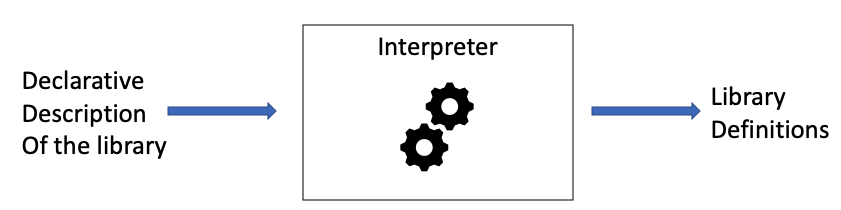
\includegraphics[scale=0.3]{figures/interpreter_small.png}
\end{figure}
\pause
\begin{itemize}
    \item Inspiration: Haskell  
\begin{onlyenv}<2>
    \begin{minted}[fontsize=\footnotesize]{haskell}
data List a = Nil | Cons a (List a) 
          deriving (Eq, Show, Ord, Read,
              -- by enabling some extensions 
                    Functor, Generic, Data,         
                    Foldable,Traversable, Lift)
    \end{minted}
\end{onlyenv}    
\begin{onlyenv}<3>
    \begin{minted}[fontsize=\footnotesize]{haskell}
data Point = Point { _x :: Double, _y :: Double }
makeLenses ''Point  
     \end{minted}
\end{onlyenv}     
\end{itemize}
\end{frame}

\begin{frame}[fragile]
\frametitle{Requirements}
\begin{enumerate}
\item A small language to represent theories without unnecessary details. 
\item Meta programs to manipulate these theories  
\item A type checker for the theories and constructions 
\item A large library of theories.
\end{enumerate}
\end{frame}

\begin{frame}[fragile]
\frametitle{Tog: Language and TypeChecker}
\begin{itemize}
    \item Dependently typed language 
    \begin{itemize}
        \item Martin L\"{o}f type theory. 
    \end{itemize}
    \item Experimental language, in the style of Agda 
\end{itemize}
\begin{minted}[fontsize=\scriptsize]{Agda}
record Monoid (A : Set) : Set where
  constructor monoid
  field
   e  : A
   op : A -> A -> A
   lunit : {x : A} -> (op e x) == x
   runit : {x : A} -> (op x e) == x
   assoc : {x y z : A} -> 
     (op x (op y z)) == (op (op x y) z)
\end{minted}
\end{frame}

\begin{frame}[fragile]
\frametitle{Approach} 
\begin{figure}
    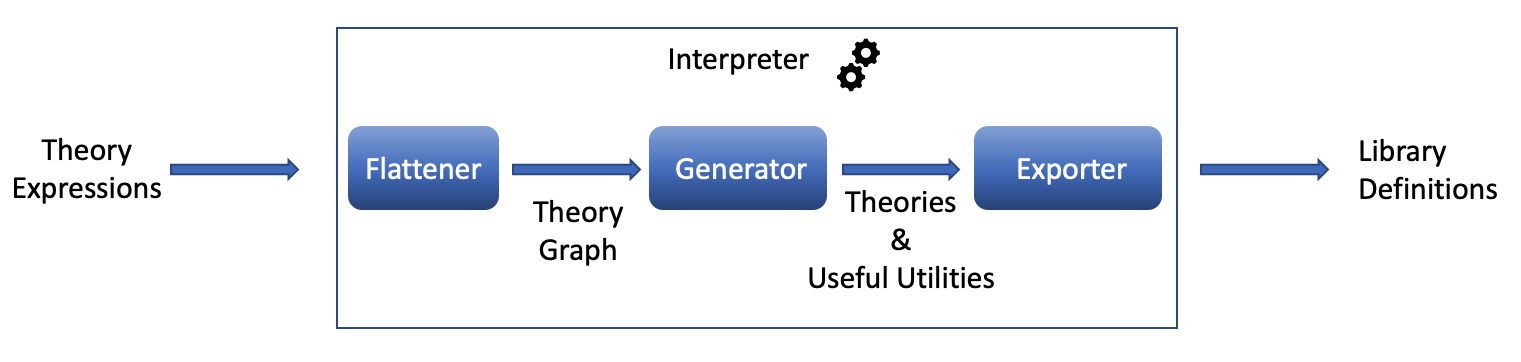
\includegraphics[scale=0.2]{figures/interpreter_detailed.png}
\end{figure}
\end{frame}

%\section{The Flattener}
\begin{frame}[fragile] 
\frametitle{The Flattener} 

%\centering{
\begin{center}
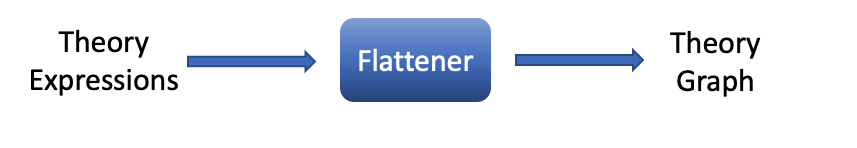
\includegraphics[scale=0.2]{figures/flattener.png}
\end{center}

\textcolor{Orange}{\textbf{Theory Graph}}



%\begin{figure}[h]
	\begin{tikzcd}[row sep=huge, column sep=scriptsize]
		&& & \verb|Pointed0| \arrow[dd,hook] & \\
		\verb|Carrier| \arrow[dd,hook] \arrow[rr,hook] & & \verb|Pointed| \arrow[ur,mapsto] & & \\ 
		& \verb|AddMagma| \arrow[rr,hook] \arrow[dd,hook]& & \verb|AddPointedMagma| 
		\arrow[rr,hook] 
		\arrow[dd,hook]& & 
		\verb|AddRightUnital|  \arrow[dd,hook]\\
		\verb|Magma| \arrow[ur,mapsto] \arrow[dd,hook]  & & 
		\verb|PointedMagma| \arrow[dd,hook] \arrow[ur,mapsto] \arrow[from=uu, crossing over] 
		\arrow[rr,hook,crossing over] \arrow[from=ll,hook, crossing over]
		& & \verb|RightUnital| \arrow[ur,mapsto] \\ 
		& \verb|AddSemigroup| \arrow[ddd,hook] & &\verb|AddLeftUnital| \arrow[rr,hook] &  & 
		\verb|AddUnital| \arrow[dddllll,hook] \\
		\verb|Semigroup|  \arrow[ddd,hook] \arrow[ur,mapsto]&  & \verb|LeftUnital| 
		\arrow[ur,mapsto] 
		\arrow[rr,hook,crossing over] &  & \verb|Unital| \arrow[dddllll,hook,crossing 
		over]\arrow[ur,mapsto] 
		\arrow[from=uu,hook,crossing over]& \\ 
		&&&& \\ 
		&  \verb|AddMonoid| &  &&\\ 
	 \verb|Monoid|  \arrow[ur,mapsto] && &&
	\end{tikzcd}
	\caption{Defining Monoid using tiny theories}
	\label{fig:cube_monoid}
%\end{figure}	

\end{frame}

\begin{frame}[fragile] 
\frametitle{The Flattener} 
\begin{center}
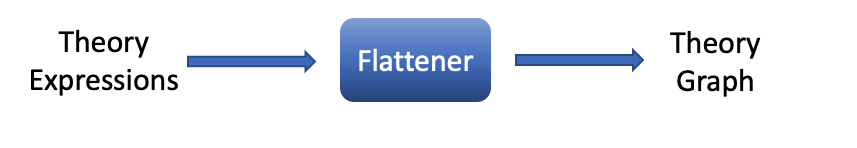
\includegraphics[scale=0.2]{figures/flattener.png}
\end{center}

\textcolor{Orange}{\textbf{Theory Expressions}} \vspace{0.2cm}

\begin{overprint}
\onslide<1>
\textbf{Extension}
\begin{columns}
\begin{column}{0.45\textwidth}
\begin{minted}[fontsize=\scriptsize]{agda}
Pointed = extend Carrier {e : A}
Magma   = extend Carrier {op : A -> A -> A}
Semigroup  = extend Magma {assoc: ...}
\end{minted}
\end{column}
\begin{column}{0.45\textwidth}



{\scriptsize
  \begin{tikzcd}[row sep=2.0em, column sep=2.5em]
    \verb|Carrier| \arrow[d,hook,blue] \arrow[r,hook,blue] & \verb|Pointed| & \\
    \verb|Magma| \arrow[d,hook,blue] & & \\
    \verb|Semigroup| & &
  \end{tikzcd}
}
\end{column}
\end{columns}

\onslide<2>
\textbf{Combine}
\begin{columns}
\begin{column}{0.45\textwidth}
\begin{minted}[fontsize=\scriptsize]{agda}
Pointed = extend Carrier {e : A}
Magma   = extend Carrier {op : A -> A -> A}
Semigroup    = 
  extend Magma {assoc: ...}
PointedMagma = 
  combine Pointed {} Magma {} 
  over Carrier
\end{minted}
\end{column}
\begin{column}{0.45\textwidth}



{\scriptsize
  \begin{tikzcd}[row sep=2.0em, column sep=2.5em]
    \verb|Carrier| \arrow[d,hook] \arrow[r,hook] \arrow[dr,hook, blue]& \verb|Pointed| \arrow[d,hook,blue]& \\
    \verb|Magma| \arrow[d,hook] \arrow[r,hook, blue] & 
    \verb|PointedMagma|  & \\
    \verb|Semigroup| && 
  \end{tikzcd}
}
\end{column}
\end{columns}

\onslide<3>
\textbf{Rename}
\begin{columns}
\begin{column}{0.45\textwidth}
\begin{minted}[fontsize=\scriptsize]{agda}
PointedZero = rename Pointed {e to 0} 
AdditiveMagma   = rename Magma {op to +} 
\end{minted}
\end{column}
\begin{column}{0.45\textwidth}



{\scriptsize
  \begin{tikzcd}[row sep=2.0em, column sep=2.5em]
    \verb|Carrier| \arrow[d,hook] \arrow[r,hook] & \verb|Pointed| \arrow[r,mapsto,blue] & \verb|PointedZero| \\
    \verb|Magma| \arrow[d,mapsto,blue] & & \\
    \verb|AdditiveMagma| & &
  \end{tikzcd}
}
\end{column}
\end{columns}
\end{overprint}
\end{frame}

\begin{frame}[fragile] 
\frametitle{The Flattener: Combinators}
{\scriptsize
  \begin{tikzcd}[row sep=2.0em, column sep=2.5em]
    \verb|Carrier| \arrow[d,hook] \arrow[r,hook] \arrow[dr,hook]& \verb|Pointed| \arrow[d,hook]& \\
    \verb|Magma| \arrow[d,hook] \arrow[r,mapsto] \arrow[rd,dotted] & 
    \verb|AdditiveMagma=(A,+)|  \arrow[d,dotted] & \\
    \verb|Semigroup=(A,op,assoc)| \arrow[r,dotted] & \verb|??| & 
  \end{tikzcd}
}
\pause 
\vspace{0.5cm}
\begin{minted}[fontsize=\scriptsize]{agda} 
AdditiveSemigroup = 
  combine AdditiveMagma {} Semigroup {op to +}
  over Magma 
\end{minted} 
\end{frame}

\begin{frame}[fragile]
\frametitle{The Flattener} 
\begin{center}
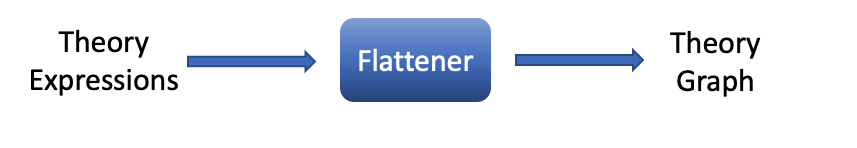
\includegraphics[scale=0.2]{figures/flattener.png}
\end{center}

\begin{overprint}
\begin{columns}
\begin{column}{0.45\textwidth}
\begin{minted}[fontsize=\scriptsize]{agda}
Pointed = extend Carrier {e : A}
Magma   = 
  extend Carrier {op : A -> A -> A}
Semigroup    = 
  extend Magma {assoc: ...}
PointedMagma = 
  combine Pointed {} Magma {} over Carrier
LeftUnital   = 
  extend PointedMagma { lunit_e : ... }
RightUnital  = 
  extend PointedMagma { runit_e : ... }
Unital = combine LeftUnital {} RightUnital {} 
         over PointedMagma
Monoid = combine Unital {} Semigroup {} over Magma
\end{minted}
\end{column}
\begin{column}{0.45\textwidth}



{\tiny
  \begin{tikzcd}[row sep=2.0em, column sep=2.5em]
    \verb|Carrier| \arrow[d,hook] \arrow[r,hook] \arrow[dr,hook]& \verb|Pointed| \arrow[d,hook]& \\
    \verb|Magma| \arrow[d,hook] \arrow[r,hook] & 
    \verb|PointedMagma|  \arrow[d,hook] \arrow[rr,hook] \arrow[drr,hook]
    & & \verb|RightUnital|  \arrow[d,hook]\\
    \verb|Semigroup| \arrow[rd,hook] & \verb|LeftUnital| \arrow[rr,hook] & &\verb|Unital| \arrow[dll,hook] & \\
   & \verb|Monoid|  & &&
  \end{tikzcd}
}
\end{column}
\end{columns}
\end{overprint}
\end{frame}

%\section{The Generator}
\begin{frame}[fragile]
\frametitle{The Generator}
\begin{minted}[escapeinside=||,mathescape=true,fontsize=\scriptsize]{haskell}
data EqTheory = EqTheory  {
  name        :: Name_   ,
  sort        :: Constr  ,  -- the carrier $\mathcal{S}$
  funcTypes   :: [Constr],  -- function symbols $\mathcal{F}$
  axioms      :: [Constr],  -- equations $\mathcal{E}$
  waist       :: Int        -- the number of parameters
}  
\end{minted}
\end{frame}

\begin{frame}[fragile] 
\frametitle{Constructions for Free!} 
\begin{tikzpicture}[node distance=2cm]
    \node(NodeName1){
\begin{lstlisting}[basicstyle=\footnotesize, escapeinside=~~]
record ~\fcolorbox{blue}{white}{Monoid \fcolorbox{red}{white}{(A : Set)}}~
      : Set where 
  e  : ~\fcolorbox{red}{white}{A}~ 
  op : ~\fcolorbox{red}{white}{A}~ -> ~\fcolorbox{red}{white}{A}~ -> ~\fcolorbox{red}{white}{A}~ 
  lunit : ...
  runit : ... 
  assoc : ...
\end{lstlisting} 
};
\node(NodeName2) [right=of NodeName1] {  % added position of second box
\begin{lstlisting}[basicstyle=\footnotesize, escapeinside=~~]
record Hom ~\fcolorbox{red}{white}{\{A1 A2 : Set\}}~ 
       ~\fcolorbox{blue}{white}{(M1 : Monoid A1) (M2 : Monoid A2)}~
       : Set where 
  hom : ~\fcolorbox{red}{white}{A1}~ -> ~\fcolorbox{red}{white}{A2}~ 
  pres-e : hom ~\fcolorbox{green}{white}{(e M1)}~ = ~\fcolorbox{green}{white}{e M2}~ 
  pres-op : {x1 x2 : A1} -> 
    hom (~\fcolorbox{green}{white}{(op M1) x1 x2}~) = 
    ~\fcolorbox{green}{white}{(op M2) (hom x1) (hom x2)} 
\end{lstlisting} };  



%\draw[red, line width=0.5mm,-{Triangle[angle=60:0.5pt 3]}] (NodeName1) -- (NodeName2);
%\draw[blue, line width=1mm,-{Triangle[angle=60:1pt 3]}] (NodeName1) -- (NodeName3);
\end{tikzpicture}

\begin{overprint}
\onslide<1>
\begin{minted}[escapeinside=||,mathescape=true,fontsize=\scriptsize]{haskell} 
homomorphism :: Eq.EqTheory -> Decl
homomorphism thry =
  let nm = "Hom" 
     i1@(|\fcolorbox{blue}{white}{n1},\fcolorbox{red}{white}{b1},\fcolorbox{green}{white}{e1}|) = Eq.eqInstance thry (Just 1)
      i2@(n2,b2,e2) = Eq.eqInstance thry (Just 2)
      fnc    = homFunc thry i1 i2
      axioms = map (presAxiom thry i1 i2 fnc) (thry ^. Eq.funcTypes)  
  in Record (mkName nm)
   (mkParams |$\$$| |\fcolorbox{red}{white}{b1 ++ b2 ++}|
               map (|$\backslash$|(n,e) -> Bind [mkArg n] e) [(|\fcolorbox{blue}{white}{n1}|,|\fcolorbox{green}{white}{e1}|),(|\fcolorbox{blue}{white}{n2}|,|\fcolorbox{green}{white}{e2}|)])}
   (RecordDeclDef setType (mkName |$\$$| nm ++ "C") (mkField |$\$$| fnc : axioms))
\end{minted} 
\end{overprint}
\end{frame}

\begin{frame}[fragile] 
\frametitle{Constructions for Free!} 
\begin{figure}
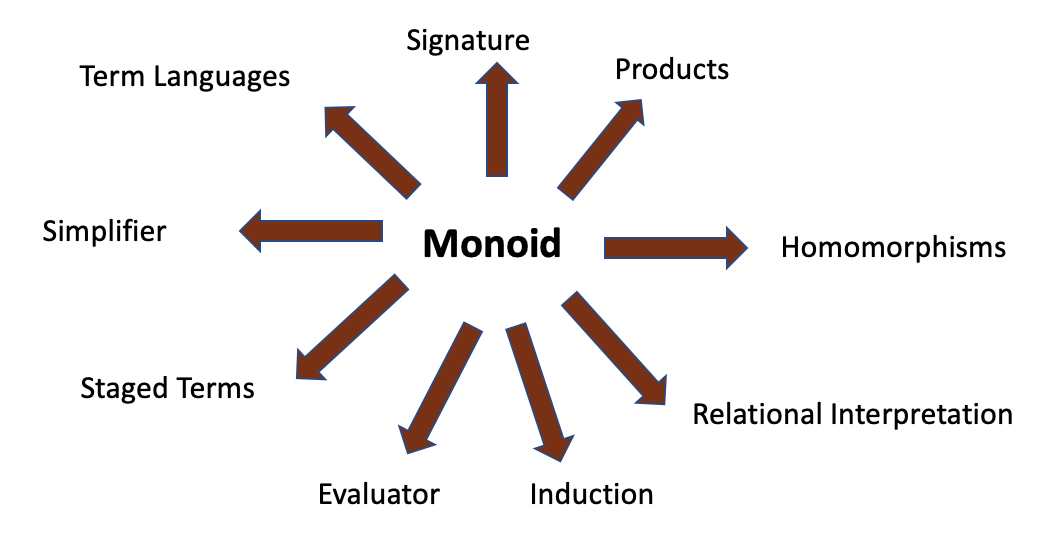
\includegraphics[scale=0.25]{figures/monoid_generation2.png}
\end{figure}
\scriptsize
Monomorphism, Isomorphism, Endomorphism, Congruence relation, Quotient algebra, Trivial subtheory, Flipped theory, Monoid action, Monoid Cosets, composition of morphisms, kernel of homomorphisms, parse trees.  
\end{frame}

%\section{The Exporter}
\begin{frame}[fragile] 
\frametitle{The Exporter} 
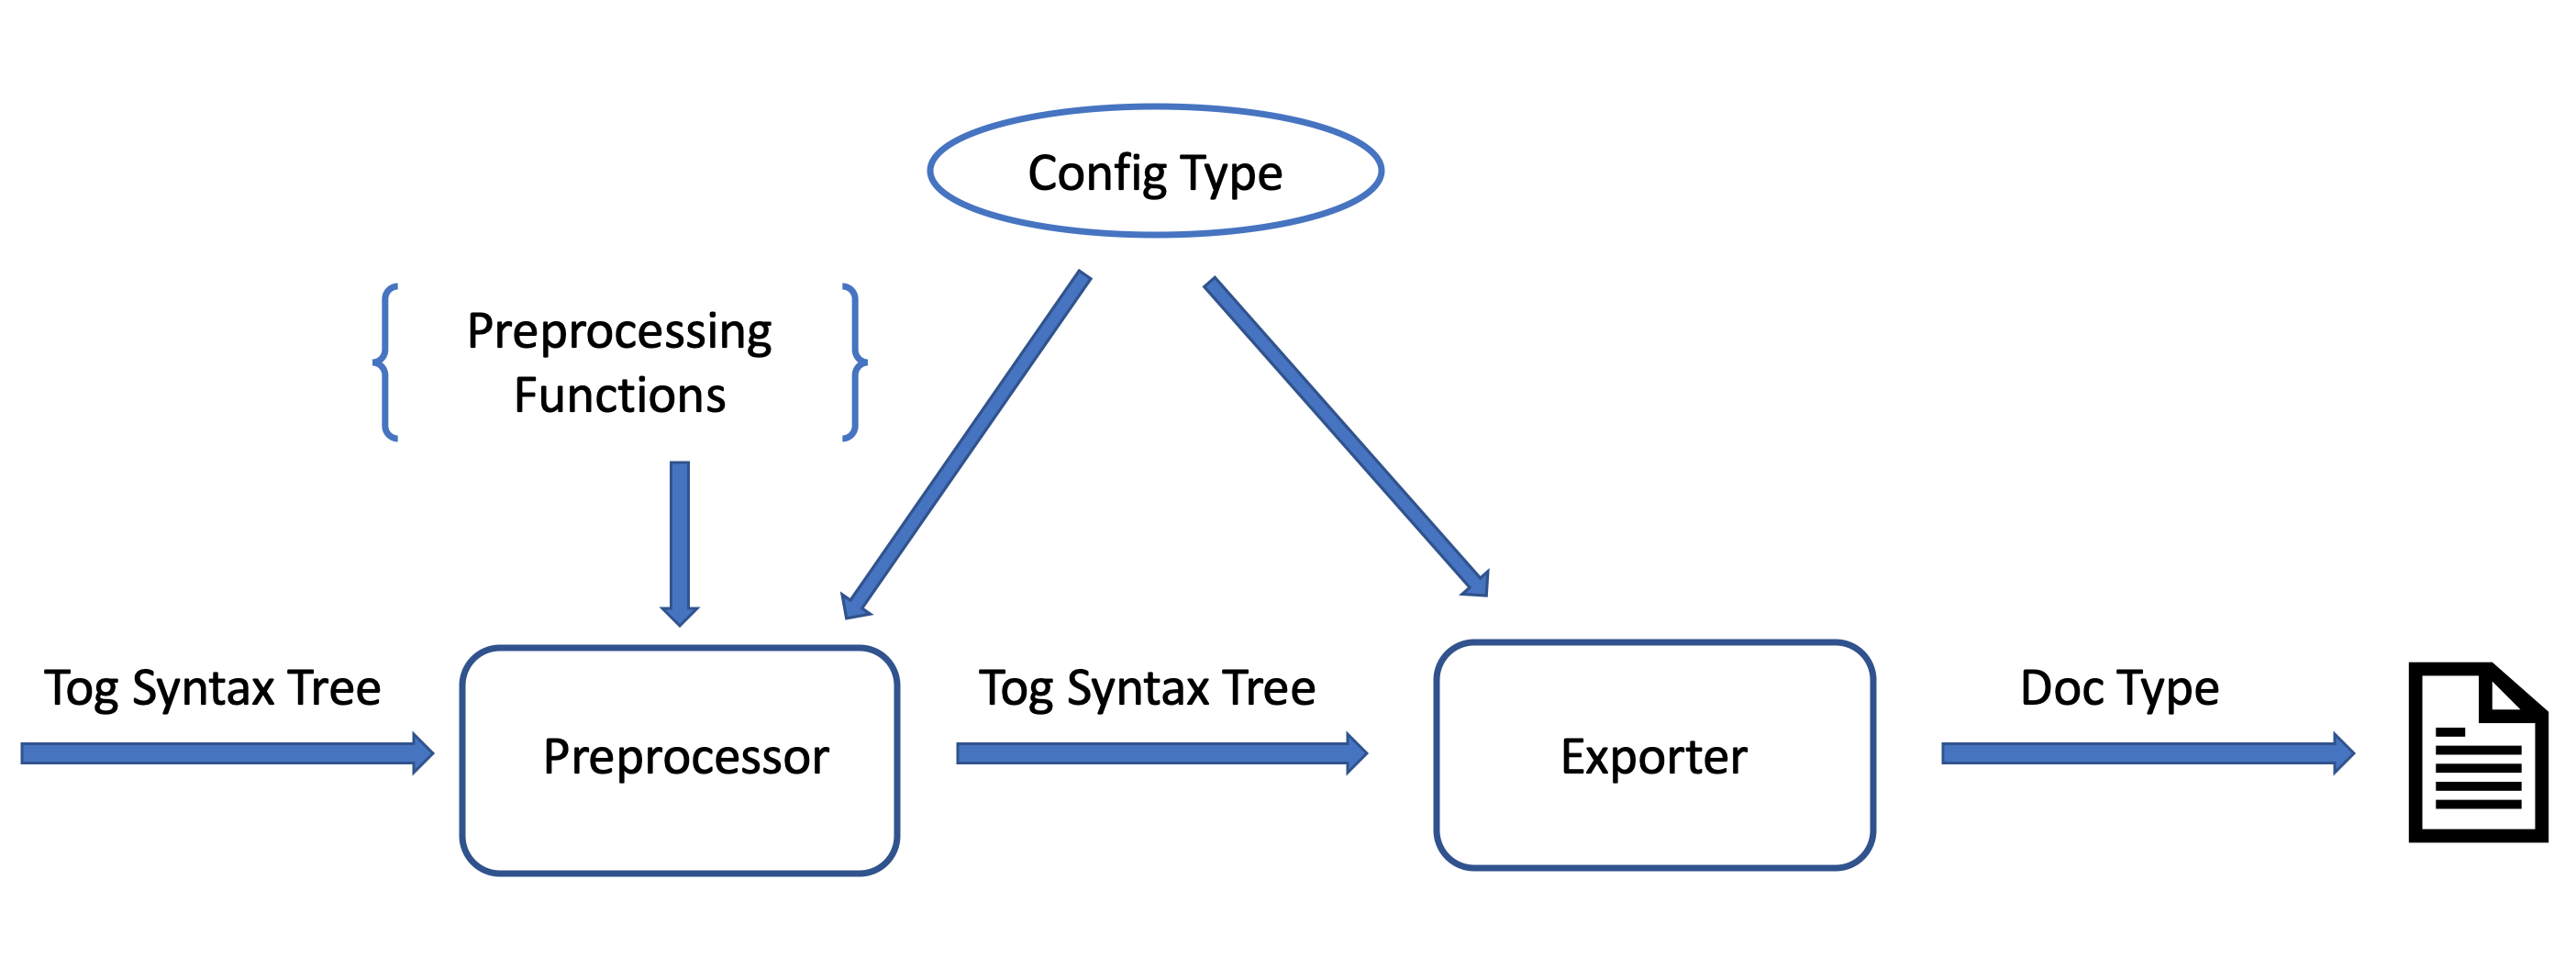
\includegraphics[scale=0.2]{../figures/exporter_arch.png}
\begin{overprint}
\onslide<1>
\textbf{Preprocessor}
\begin{itemize}
\item Universes 
\item Prelude Definitions 
\end{itemize}
\onslide<2>
\textbf{Exporter}
\begin{minted}[fontsize=\scriptsize]{haskell} 
class Export a where
  export :: Config -> a -> Doc
\end{minted} 
\end{overprint}
\end{frame}

\begin{frame}[fragile] 
\frametitle{Results}
Starting with \textbf{\textcolor{Orange}{227}} theory expressions:
\begin{itemize}
\item \textcolor{Orange}{\textbf{5092}} library definitions. 
\item \textcolor{Orange}{\textbf{32,459}} lines of code. 
\item Exported to \textcolor{Orange}{\textbf{Lean}}, \textcolor{Orange}{\textbf{Agda}} (flat and predicate style theories).
\end{itemize}
\end{frame}

%\section{Conclusion and Future Work}
\begin{frame}[fragile] 
\frametitle{Conclusion} 
Develop a generative approach to library building 
\begin{itemize}
\item Highlight the redundancy in libraries formalizing the algebraic hierarchy.
\item Build a library of $227$ theories describing the algebraic hierarchy using theory combinators.
\item Compile a list of structures that can be generated from theory presentations.
\item Generate some of these constructions in Tog, a small implementation of a dependently typed language.
\item Export this implementation to Agda and Lean.
\end{itemize}
\end{frame}

\begin{frame}[fragile] 
\frametitle{Future Work}
\begin{itemize}
\item Proof assistants as \textcolor{Orange}{\textbf{program families}}. 
\begin{itemize}
\item better understanding how design decisions affect theory presentations 
\item staged exporter to multiple proof assistants 
\end{itemize}
\pause
\vspace{0.5cm}
\item a \textcolor{Orange}{\textbf{DSL}} for library development. 
\vspace{0.2cm}
\begin{minted}[escapeinside=||,mathescape,fontsize=\scriptsize]{Haskell}
Monoid = combine Unital and Semigroup over Magma
         generate Homomorphism, OpenTerms, Simplifier
         using (waist=1,eq="=")
         export_to lean
\end{minted}
\pause 
\vspace{0.5cm}
\item Generalizing the approach to \textcolor{Orange}{\textbf{generalized algebraic theories}}.
\end{itemize}
\end{frame} 

\plain{Thank You!} 

\end{document}